\section{Fusion}
Kärnreaktorer har ni säkert hört talas om. Oftast funkar dessa genom att klyva atomkärnor, det vill säga utföra \emph{fission}. Stjärnor gör något liknande, men de sätter ihop atomkärnor i stället för att klyva isär dem. Detta heter \emph{fusion}. Det krävs väldigt höga tryck och temperaturer för att möjliggöra fusion, men i vissa fall ger processen mer energi ut än som sattes in, vilket är det som bland annat möjliggör stjärnor.

Både fission och fusion fungerar eftersom olika atomer har olika \emph{bindningsenergi}. Det finns nämligen en viss energi som krävs för att se till att nukleonerna i atomkärnan inte flyger iväg. Bindningsenergin är också förvånansvärt stor. Vi har svårt att mäta den direkt, men man kan använda Einsteins materia-energiekvivalens:
\begin{equation}
    E = mc^2
    \label{eq:emc2}
\end{equation}
i stället.

Ekvivalensen säger att den totala energin lagrat i ett visst föremål är lika med dess massa gånger ljusets hastighet i kvadrat. Med hjälp av detta kan vi observera skillnaden i energi mellan samma molekyl i olika tillstånd. Till exempel kommer energin för 2 lösa protoner (\ce{2p+}) och 2 lösa neutroner (\ce{2n}) vara större än dessa sammansatta för att bilda en \ce{^2_4He^2+} kärna som ni kan se i \cref{tab:helium-energy}. En elektrons massa är försumbart liten i detta sammanhang, och deltar därför inte i beräkningarna.

Denna relation kan även tillämpas för skillnaden mellan två fria atomkärnor och en större atomkärna bildad genom att \emph{fusionera} --- sätta samman till ett --- de två kärnorna. För lika par av grundämnen gäller det att deras fusionsprodukt alltid har lite lägre energi än de skiljda upp till järnatomen. Efter järn har fusionsprodukten av ett likt par grundämnen lite mer energi fusionerat än separat.

Detta innebär i slutändan att fusionsreaktioner av lika atompar ger ett energiöverskott för grundämnen upp till järn. Detta överskott blir till värme. Den extra energin är ganska liten jämfört med energin som krävs för att trycka ihop atomkärnorna men är inte försumbar i stora skalor med många atomer samtidigt. För fusion av olika par är frågan mer komplicerad, men generellt sett är det energivinst även där upp till järn.

\subsection{Fusion i stjärnor}
Tack vare stjärnors stora tryck, och temperatur, möjliggör en stjärna med stor nog massa fusion av grundämnen. Gränsen för att kunna fusionerna väte till helium ligger på \qty{\sim 0.08}{\Mo}\footnote{Källa: \textcolor{blue}{\url{https://sites.uni.edu/morgans/astro/course/Notes/section2/fusion.html}}} (solmassor). Sedan finns det en skala för hur mycket energi, och därav massa hos stjärnan, krävs för att fusionera varje element. Ju större stjärna, desto högre tryck från tyngdkraften, alltså desto högre värme. Till slut når man kisel till järn fusion, och därefter är energipositiv fusion omöjlig. Detta innebär också att järn inte längre kan fusioneras av stjärnan.

Fusion i stjärnor är inte lika perfekt som min tidigare förklaring antydde. Det är sällan lika atompar som bara sådär slås samman. Exempelvis finns proton-proton fusion som skapar helium från väten som ni kan se i \cref{fig:proton-proton}. Det är denna process som just nu pågår i solen.

\begin{figure}
    \centering
    \includegraphics[width=0.35\textwidth]{img/Fusion_in_the_Sun.png}
    \caption{Proton-proton fusion.}
    \label{fig:proton-proton}
\end{figure}

\begin{table}[b]
    \def\arraystretch{1.5}
    \centering
    \caption{Energin för heliums beståndsdelar och dess kärna.}
    \label{tab:helium-energy}
    \begin{tabular}{c|c|c}
        \textbf{Sak} & \textbf{Massa (kg)} & \textbf{Energi (J)} \\\toprule
        \ce{2p+ + 2n} & \qty{6.696e-27}{kg} & \qty{6.018e-10}{J}\\
        \ce{^2_4He^2+} & \qty{6.646e-27}{kg} & \qty{5.974e-10}{J} \\\bottomrule
        \textbf{Differens} & \qty{5e-30}{kg} & \qty{4.4e-12}{J}

    \end{tabular}
\end{table}

\section{Stjärnornas anatomi}
En stjärna är i grund och botten en boll av gas. Först och främst består dem av väte (\ce{H}) och helium (\ce{He}). De innehåller dock ämnen hela vägen upp till järn (\ce{Fe}) i periodiska systemet (se \vref{fig:periodic-table} för ett periodiskt system).

Deras inre struktur kan liknas till en lök. I mitten finns kärnan, sedan har man lager av olika gaser och plasman för att sista komma ut till yttersta skicket av gas som vi ser utifrån. Ett diagram återfinns i \cref{fig:star-anatomy}. Denna uppdelning beror på hur stjärnor fungerar.

\begin{figure}[h!]
    \centering
    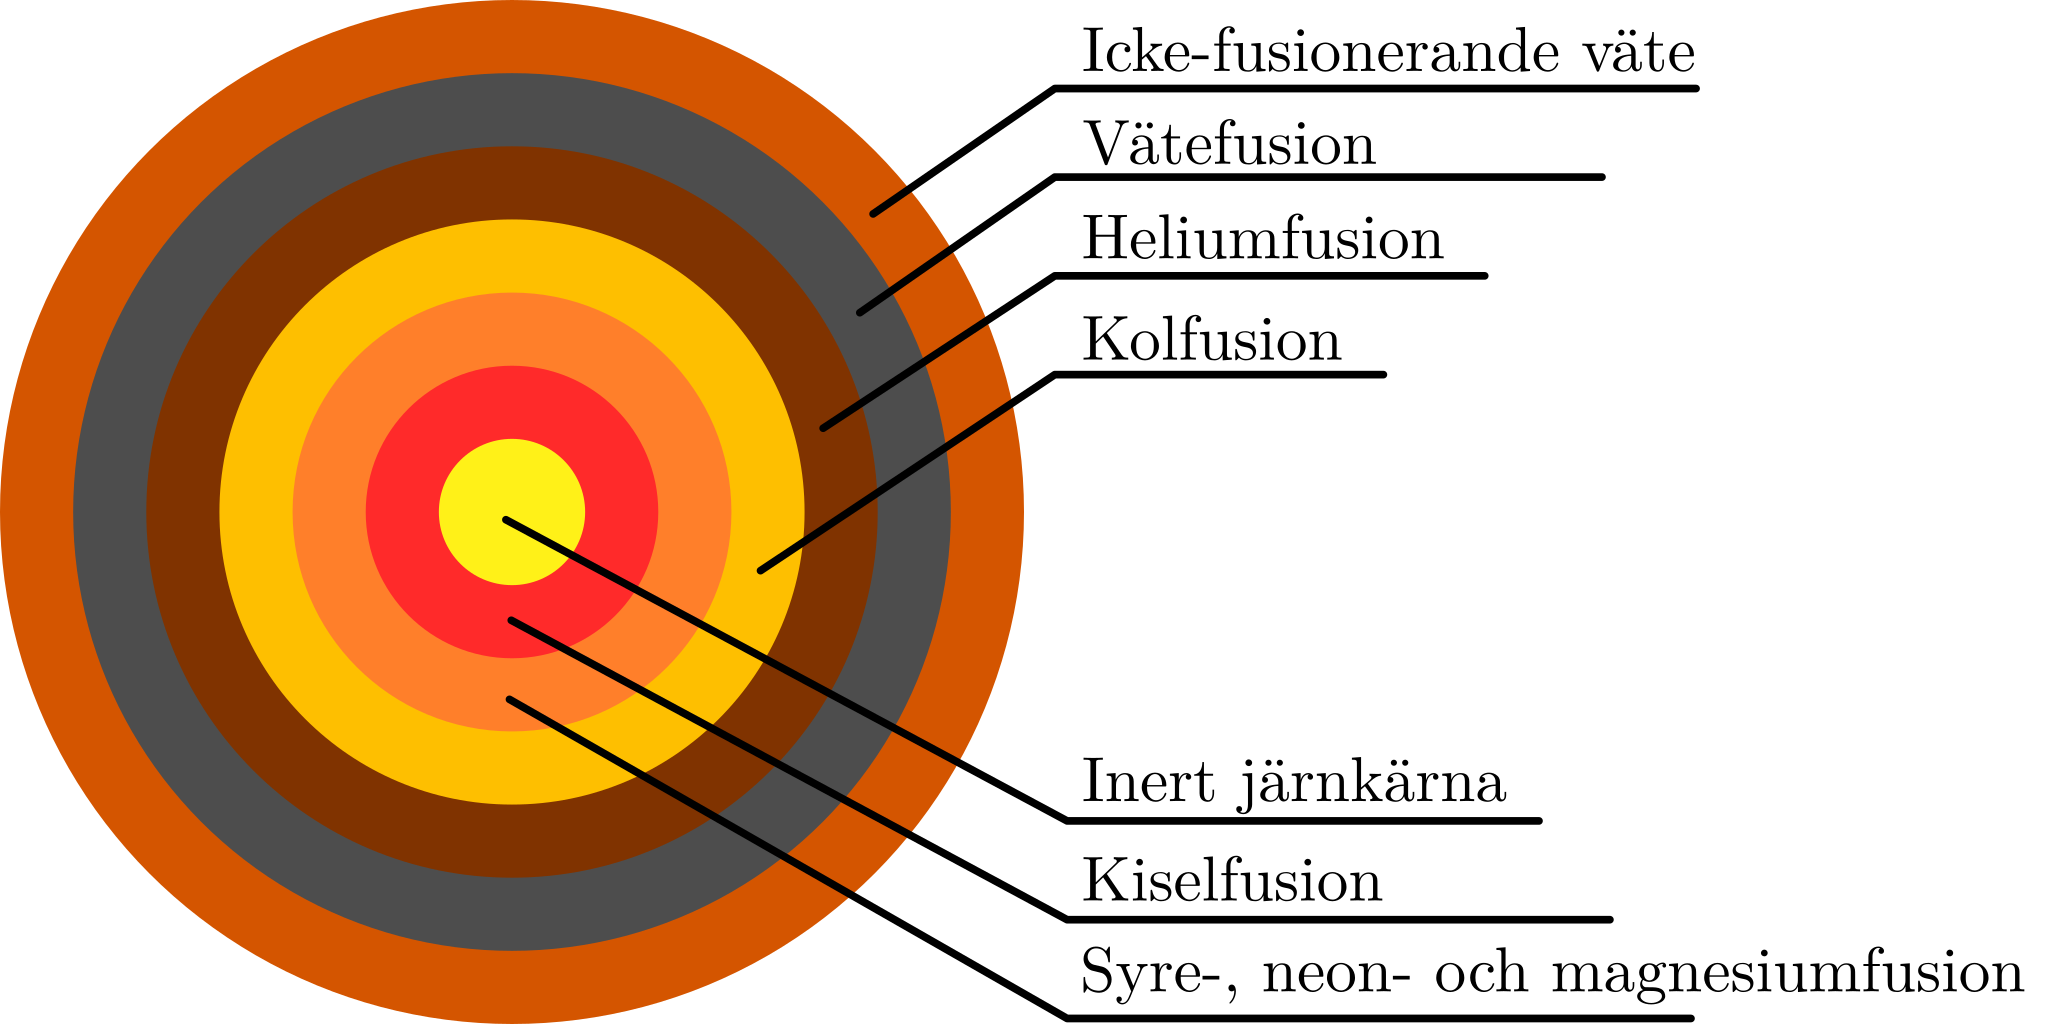
\includegraphics[width=0.8\textwidth]{img/star.png}
    \caption{En gammal stjärnas inre struktur.}
    \label{fig:star-anatomy}
\end{figure}